%
%	\subsection{Paramétrisation et relation source-récepteur}
%	

%	
%	
%	\begin{equation}
%		\label{eq_relation_SR_non_parametrique}
%		\VecObs = \bm{H}\VecSigma + \bm{\varepsilon}
%	\end{equation}
%	

%	
%	Dans le cas particulier d'une source ponctuelle on peut, dans l'équation \eqref{eq_relation_SR_non_parametrique}, substituer $\VecSigma$ par un profil d'émission $\VecSigma$ issu d'un unique point du domaine spatial considéré. En procédant ainsi, il n'est plus nécessaire de définir arbitrairement un maillage conditionné par $N_x, N_y, N_z$  sur le domaine. De plus, la dimension du problème se réduit à estimer un point de l'espace et son profil temporel associé, soit $T_s + 3$ inconnues, contrairement au cas général où il faut retrouver l'intégralité du champ d'émission, soit $N_xN_yN_zT_s$ inconnues.\\
%	
%		
	\section{Estimation du terme source: un état de l'art}
	\label{section_etat_art_STE}
	
	\subsection{Une brève introduction aux problèmes inverses}
	Le domaine des problèmes inverses constitue un vaste champ de la littérature scientifique, et de nombreux travaux y ont été menés. En pratique, résoudre un problème inverse revient à reconstituer un signal, une image, ou plus généralement une donnée non-observable à partir de mesures existantes, appelées observations.
	Cette approche est duale à celle du problème direct où, à partir d'un signal ou d'un ensemble de paramètres initiaux, on cherche à en calculer les effets après une transformation donnée (figure \ref{fig_diagramme_direct_inverse}).
	De nombreux domaines théoriques et pratiques font appel aux méthodes inverses. Le lecteur pourra trouver une revue complète de ces applications dans \cite{Tarantola2004}, on peut en citer quelques exemples tels que la géophysique \cite{Backus1967}, l'acoustique \cite{Kirsch1988}, l'imagerie satellite \cite{Park2003} et médicale \cite{Arridge1999}, les transferts thermiques \cite{McCormik1992} ou encore la finance quantitative \cite{Dembo1999}.\\
	
	\begin{figure}
		\centering
		\includegraphics[scale=0.5]{diagramme_direct_inverse.png}
		\caption{Schéma de principe illustrant la dualité entre problèmes direct et inverse.}
		\label{fig_diagramme_direct_inverse}
	\end{figure}
	
	
	En dispersion atmosphérique, le problème direct peut ainsi se traduire par la donnée des paramètres de la source au modèle de dispersion, qui va produire le champ de concentration résultant. Cela revient bien à définir le problème inverse comme étant la reconstruction des paramètres de la source à partir des mesures de concentrations aux capteurs. Nous décrivons dans les paragraphes suivants les différentes approches existant dans la littérature qui permettent de résoudre ce problème. Des éléments complémentaires sur la question sont également disponibles dans \cite{Rao2007}. Dans un souci de brièveté, par la suite nous qualifierons de "problèmes STE" (\textit{source term estimation}) toutes les études de cas visant à estimer les paramètres d'une ou de plusieurs sources inconnues.\\
	
	
 \subsection{{Rétro-transport et modèles rétrogrades}}
 
 Une première possibilité consiste à étudier le problème dual associé à l'équation d'advection-diffusion  \eqref{eqn_advection_diffusion}, en inversant la flèche du temps, et par conséquent la direction du vent.  Par le principe de symétrie présenté dans \cite{Hourdin2006a}, on peut alors introduire la notion de \textit{rétro-transport} ou \textit{backtracking} en  réécrivant l'équation d'advection-diffusion sous la forme : 
 
 \begin{equation}
 \label{eqn_advection_diffusion_backward}
 \dfrac{-\partial C^*}{\partial t} - \nabla \cdot(C^*\bm{\vec{u}}) = \nabla \cdot (\bm{K}\nabla C^*) + \VecObs
 \end{equation}
 
 où $C^*$ est un champ de concentrations conjuguées, ou \textit{rétro-concentrations}, dont les valeurs sont obtenues par des rétro-rejets virtuels depuis les capteurs vers la source. Le modèle de dispersion associé à cette démarche duale est alors appelé {\textit{modèle de rétro-dispersion}, ou \textit{modèle rétrograde}}. Cette démarche revient ainsi à transformer le champ d'émission {obtenu par l'équation \eqref{eqn_advection_diffusion}} en un champ de rétro-émissions issues des capteurs, comme illustré sur les figures \ref{schema_probleme_direct} et \ref{schema_probleme_inverse}, et ainsi fournir une estimation du terme source.\\
 
 \begin{figure}[h]
 	\begin{subfigure}{0.5\textwidth}
 		\includegraphics[scale=0.6]{schema_probleme_direct.png}
 		\caption{Approche orientée source}
 		\label{schema_probleme_direct}
 	\end{subfigure}
 	\begin{subfigure}{0.5\textwidth}
 		\includegraphics[scale=0.2]{schema_probleme_inverse.png}
 		\caption{Approche orientée récepteur}
 		\label{schema_probleme_inverse}
 	\end{subfigure}
 	\caption{Exemple illustrant la relation entre une source unique $S$ et trois capteurs $R_1,R_2,R_3$ sur un problème en deux dimensions pour les approches en "direct" (\ref{schema_probleme_direct}) et en "adjoint" (\ref{schema_probleme_inverse}). }
 \end{figure}
 
 Dans \cite{Flesch1995}, un modèle {rétrograde} lagrangien est construit pour estimer le profil de rejet d'une source surfacique.  Cette méthode est également appliquée dans \cite{Pudykiewicz1998}, où la position et l'intensité du terme source de Tchernobyl sont reconstruits. De même, dans \cite{Hourdin2006b} le principe du \textit{backtracking} est appliqué à un modèle eulérien pour retrouver la source de la campagne ETEX\footnote{L’expérience \textit{European Tracer EXperiment 1} (ETEX-1), menée en 1994,  a consisté à mesurer et étudier l'impact à l'échelle européenne de rejets de gaz traceurs passifs émis depuis une source située dans la ville de Monterfil, en Bretagne.}.\\
 
 \subsection{Formulation linéaire du problème et optimisation}
 \label{subsection_MCO}
 
Le modèle direct de simulation des concentrations résultant d'un rejet de polluant peut être décrit de façon linéaire. Pour cela, on définit de façon arbitraire un maillage dans le temps et l'espace qui couvre respectivement la période d'observation et le domaine spatial considérés. En pratique, cela revient à discrétiser l'espace en $N_xN_yN_z$ points, chaque point étant associé à un profil d'émission de longueur $T_s$. Dans un tel contexte, le terme source est défini comme un vecteur $\VecSigma \in \mathbb{R}^{N_\VecSigma}$ (où $N_\VecSigma = N_xN_yN_zT_s$). Il est ainsi possible de lier les observations générées par le modèle et le vecteur source $\VecSigma$ par la formule suivante, appelée \textit{relation source-récepteur}:

\begin{equation}
	\label{eq_relation_SR_non_parametrique}
	\VecObs = \bm{H}\VecSigma + \bm{\varepsilon}
\end{equation}
où $\VecObs \in \mathbb{R}^m$ représente le vecteur des observations, $\VecSigma \in \mathbb{R}^{N_\VecSigma}$ la source discrétisée et $\bm{H} \in \mathbb{R}^{m \times N_\VecSigma}$  la \textit{matrice de transfert}. Le rôle de $\bm{H}$ est d'assurer la projection depuis l'espace $\mathbb{R}^{N_\VecSigma}$  de la source vers l'espace $\mathbb{R}^m$ des observations grâce à l'utilisation d'un modèle de dispersion atmosphérique. $\bm{\varepsilon} \in \mathbb{R}^m$ est le vecteur des erreurs d'observation, et prend en compte les erreurs de mesure, de représentativité et de modèle. \\

Retrouver le terme $\VecSigma$ dans l'équation \eqref{eq_relation_SR_non_parametrique} revient alors à résoudre un problème inverse linéaire: il existe pour cela différentes méthodes que nous détaillons ci-après.

\subsubsection{Définition de la fonction-coût à optimiser}

L'équation \eqref{eq_relation_SR_non_parametrique} peut être réécrite sous la forme : 
 
 \begin{equation}
 \VecObs = \widehat{\VecObs} + \VecErreur
 \label{eq_relation_SR_nonparam_simple}
 \end{equation}

où $\widehat{\VecObs} = \MatH \VecSigma$ est l'approximation des observations $\VecObs$ par le processus de modélisation. On voit bien que dans le cas parfait où ce dernier reproduit exactement les observations attendues, on a $\VecErreur = 0$ et par suite $\widehat{\VecObs} = \VecObs$. Le fait de chercher la valeur $\VecSigma$ pour laquelle $\widehat{\VecObs}$ se rapproche le plus de $\VecObs$ permet ainsi de définir le problème STE sous la forme d'une minimisation de l'erreur $\VecErreur$: on définit pour cela une fonction-coût qui s'écrit : 

\begin{equation}
\CostF(\VecSigma) = ||\VecObs - \MatH \VecSigma||_p = ||\VecObs- \widehat{\VecObs}||_p
\label{eq_cost_function_definition}
\end{equation}
où $||\cdot||_p$ désigne une norme $L_p$ arbitrairement choisie. La résolution du problème STE se traduit alors par la minimisation de cette fonction-coût:

\begin{equation}
\widehat{\VecSigma} = \argmin_\VecSigma \mathcal{J}(\VecSigma)
\label{eq_argmin_cost_function}
\end{equation}
où $\widehat{\VecSigma}$ est l'estimation du terme source recherchée.

\subsubsection{Minimisation d'une fonction-coût quadratique}

Une des approches les plus courantes pour résoudre l'équation \eqref{eq_argmin_cost_function} consiste à choisir $p=2$, autrement dit à minimiser l'écart quadratique entre les observations $\VecObs$ et les données générées par le modèle direct. Concrètement, cela revient à optimiser la fonction-coût suivante:

\begin{equation}
\CostF_{2}(\VecSigma) = ||\VecObs - \MatH \VecSigma ||_2^2
\label{eq_cost_MCO}
\end{equation}

Le fait de minimiser $\CostF_2$ revient à appliquer la méthode des \textit{moindres carrés} pour résoudre le problème inverse. 

Le terme d'erreur que nous cherchons à minimiser est une combinaison des différentes sources d'incertitudes existantes (mesure, représentativité, modèle). Comme il est difficile de quantifier les contributions respectives de ces dernières, on peut invoquer le principe du maximum d'entropie pour définir la représentation statistique de l'ensemble des incertitudes comme étant un bruit gaussien centré et de matrice de covariance $\MatR$ : 
\begin{equation}
\VecErreur \sim \mathcal{N}(0,\MatR)
\label{eq_bruit_obs}
\end{equation}

Dans le cadre de statistiques gaussiennes, la fonction-coût peut alors s'écrire sous la forme suivante \cite{Winiarek2011}:

\begin{equation}
\mathcal{J}_2(\VecSigma) = \dfrac{1}{2}(\VecObs - \MatH \VecSigma)^T \MatR^{-1}(\VecObs - \MatH\VecSigma)
\label{eq_cost_forme2}
\end{equation}

{Dans l'hypothèse où les éléments du vecteur de bruit sont indépendants et identiquement distribués, alors la matrice $\MatB$ est diagonale:}
	
	\begin{equation}
	{
		\MatB = \sigma_R^2 \MatId
	}
	\end{equation}
{où $\sigma_R^2$ est la variance d'erreur.} Plusieurs travaux dans la littérature ont recours a cette formulation: \\
\begin{itemize}
	\item Dans \cite{Kathirgamanathan2002}, un point source instantané est estimé à l'aide d'une méthode des moindres carrés, cette source étant caractérisée par sa masse totale émise, sa position et son instant d'émission. L'étude qui y est menée met notamment l'accent sur l'influence du dimensionnement du réseau de capteurs sur la performance de la reconstruction : au moins trois points de mesure sont nécessaires, et la distance entre les différents capteurs influe sur la qualité de l'estimation.\\
	
	\item Dans \cite{Ryall2001}, ce sont des zones d'émission plus grandes qui sont estimées pour des rejets de gaz à effet de serre sur plusieurs années. \\
	
	\item Dans \cite{Matthes2005}, une approche en deux temps est formulée afin de résoudre un problème de complexité proportionnellement croissante au nombre de capteurs. Dans une première étape, les mesures individuelles de chaque capteur produisent des ensembles de positions probables pour la source. Dans un deuxième temps, ces ensembles sont comparés pour estimer la meilleure position en faisant varier l'intensité de la source à retrouver. \\
	
	\item  Dans \cite{Robertson1998}, l'inversion est faite dans le cadre de l'assimilation de données: cette méthodologie permet de corriger de façon variationnelle les paramètres du modèle de dispersion selon une boucle de rétro-action basée sur des observations. Très utilisée en météorologie, l'assimilation de données agit en deux temps selon un principe de "prévision-correction", et itère sur le cycle suivant:
	\begin{enumerate}
		\item  on calcule d'abord une ébauche de l'état à l'instant présent $t$, en appliquant un modèle de prévision en $t-1$,
		\item  on exploite ensuite les observations disponibles à l'instant $t$ pour corriger les paramètres du modèle en les comparant avec l'ébauche. \\
	\end{enumerate}
	
	 \item \cite{Issartel2005} mentionne le principe d'\textit{illumination}, qui est une mesure quantitative de la représentativité des mesures dans le temps et l'espace. Dans le cadre d'un modèle adjoint, l'illumination permet ainsi de caractériser des zones qui ne sont pas forcément couvertes par les rétro-émissions issues des capteurs, par exemple si la zone considérée est relativement éloignée {de tout point de mesure}. Cependant, si l'information d'illumination est utilisée pour inverser un terme source, alors elle aura tendance à fortement favoriser les solutions proches des capteurs. Pour compenser ce problème, une phase de \textit{renormalisation} est introduite (\cite{Issartel2007} et \cite{Sharan2009}) pour équilibrer l'information apportée par chacun des capteurs. D'abord utilisée à grande échelle, cette méthodologie a récemment été validée à l'échelle locale dans \cite{Singh2014}, et dans un contexte urbain par \cite{Kumar2015}. \\

\end{itemize}

\subsubsection{Régularisations}

Bien souvent, le nombre d'observations à notre disposition est limité, à cause par exemple d'un faible nombre de capteurs ou d'une mauvaise représentativité temporelle dans les mesures fournies par ces derniers. Dans de telles situations, le problème inverse peut admettre une infinité de solutions, et ainsi devenir \textit{mal-posé}. Rappelons qu'un problème \textit{bien posé} au sens de Hadamard \cite{Hadamard1902} désigne un modèle mathématique dont la solution existe, est unique, et dépend de façon continue des données. A l'inverse, un problème mal-posé déroge à au moins une des règles précédemment citées. \\

De nombreux problèmes physiques sont intrinsèquement mal-posés, et des solutions existent pour les \textit{régulariser}, c'est-à-dire leur appliquer une transformation qui permet de revenir à un problème bien posé. Parmi ces méthodes, la \textit{régularisation de Tikhonov} \cite{Tikhonov1963} est la plus fréquemment employée: elle consiste à ajouter un terme $\lambda_B ||\VecSigmaB||_2$ dit \textit{régularisant} à l'expression de la fonction-coût $\CostF_2$, qui devient alors:

 \begin{equation}
 {
 \mathcal{J}_{2_B}(\VecSigma) = ||\VecObs - \MatH \VecSigma||_2^2 + \lambda_B ||\VecSigma||_2
 \label{eq_cost_MCO_reg}
}
 \end{equation}
 
 Le rôle du terme régularisant est de pénaliser les solutions indésirables, afin de garantir le critère d'unicité de la solution du problème inverse.  Dans le cas des statistiques gaussiennes, l'erreur  $\VecSigma - \VecSigmaB$ suit également une loi normale centrée, de matrice de covariance $\MatB$:
  
  \begin{equation}
  (\VecSigma - \VecSigmaB) \sim \mathcal{N}(0,\MatB)
  \label{eq_erreur_ebauche}
  \end{equation}
  
  L'équation \eqref{eq_cost_forme2} devient alors \cite{Winiarek2011}: 
 
\begin{equation}
\mathcal{J}_{2_B}(\VecSigma) = \dfrac{1}{2}(\VecObs - \MatH \VecSigma)^T \MatR^{-1}(\VecObs - \MatH\VecSigma) + \dfrac{1}{2}(\VecSigma - \VecSigmaB)^T\MatB^{-1}(\VecSigma - {\VecSigma_b})
\label{eq_cost_reg_forme2}
\end{equation}

Dans la littérature des méthodes d'estimation du terme source, le terme régularisant est qualifié d'\textit{ébauche}, de \textit{first-guess}, ou encore de \textit{background}. Les travaux présentés dans \cite{Winiarek2012} introduisent une approche basée sur la résolution de l'équation \eqref{eq_cost_reg_forme2} via la méthode du \textit{Best Linear Unbiased Estimator} (BLUE), qui vise à annuler le gradient de la fonction-coût cible. Une approche similaire est proposée par \cite{Saunier2013}, élaborant une reconstruction du terme source de l'accident de Fukushima en deux temps. Tout d'abord, une première fonction-coût est minimisée pour estimer la période du rejet, puis tenant compte de cette contrainte, une seconde fonction-coût est optimisée pour retrouver la localisation de la source. 

Il est intéressant de remarquer que l'équation \eqref{eq_cost_reg_forme2} correspond à celle de la méthode d'assimilation variationnelle de données 3D-var \cite{Courtier1998}. La vision de ce type d'estimation correspond  ainsi à celle de l'assimilation des concentrations mesurées par les capteurs dans le but de reconstruire un état inconnu, qui est ici le champ d'émission de la source recherchée. Notons également que des études ont été menées dans le cadre de statistiques non-gaussiennes, en particulier dans les cas où on cherche à caractériser l'ébauche suivant certaines hypothèses spécifiques \cite{Bocquet2005a}. Ainsi, les auteurs de \cite{Krysta2007} font l'hypothèse d'une source ponctuelle et instantanée pour définir une forme particulière d'ébauche, et utilisent un principe de maximum d'entropie sur la moyenne \cite{Jaynes1957} pour réécrire la fonction-coût et en dériver un estimateur approprié pour la source qu'ils recherchent.\\

Il peut exister des situations où les observations prennent l'allure de \textit{signaux parcimonieux} (ou \textit{sparse signals}), autrement dit elles sont décrites par un très faible nombre de valeurs non-nulles sur l'intervalle temporel de mesure. Pour tenir compte de cela, l'équation \eqref{eq_cost_MCO} est modifiée, et c'est cette fois un terme régularisant sous une norme $L_1$ qui est utilisé: 

\begin{equation}
\mathcal{J}_{2_L} = ||\VecObs - \MatH\VecSigma||_2^2 + \lambda_L ||\VecSigma||_1
\label{eq_MCO_L1}
\end{equation}

Une application de cette approche à la reconstruction de sources multiples est présenté dans \cite{Cheng2008}, où la régularisation $L_1$ est justifiée par la nature parcimonieuse du vecteur d'état à estimer. Une autre étude, menée dans \cite{Martinez2013} porte sur la modélisation des rejets de xénon durant l'incident de Fukushima sous la forme de brèves impulsions (ou \textit{short bursts}), fournissant ainsi un cadre approprié à la régularisation $L_1$.

\subsubsection{Une vision probabiliste du problème d'optimisation}

Il est possible d'établir une analogie entre les méthodes d'optimisation précédemment mentionnées et les approches se basant sur des calculs de lois de probabilité.

En effet, dans un cadre probabiliste, {l'optimisation sans terme régularisant est équivalente à la résolution d'un} problème de \textit{maximum de vraisemblance}. En pratique, le fait de minimiser la fonction-coût $\CostF_2$ revient ainsi à déterminer la grandeur suivante:

\begin{equation}
{
\widehat{\VecSigma_2} = \argmax_\VecSigma~ \log p(\VecObs | \VecSigma)
\label{eq_ML_MCO}
}
\end{equation}
où $p(\VecObs | \VecSigma)$ est la vraisemblance des observations pour un terme source donné. \\

De même, le fait de régulariser la fonction-coût par l'ajout d'un terme d'ébauche revient à adopter une démarche \textit{bayésienne}\footnote{Nous décrirons plus en détail les principes fondamentaux de la statistique bayésienne dans le prochain chapitre.}, où le terme régularisant représente une information a priori $p(\VecSigma)$, et l'estimateur recherché devient alors le maximum de la loi a posteriori de $\VecSigma$: 

\begin{equation}
{
\begin{split}
\widehat{\VecSigma_{2_B}} &= \argmax_\VecSigma~ \log p(\VecSigma | \VecObs) \\
 &= \argmax_ \VecSigma \left(\log p(\VecObs | \VecSigma) + \log p(\VecSigma)\right)
\label{eq_MAP}
\end{split}
}
\end{equation}

{
Dans le cas de la régularisation $L_1$ présenté à l'équation \eqref{eq_MCO_L1}, la démarche est équivalente à l'introduction d'une information a priori de parcimonie sous la forme d'une loi laplacienne pour $p(\VecSigma)$. Cette démarche de maximum a posteriori est alors équivalente à l'estimateur \textit{Least Absolute Shrinkage and Selection Operator} (LASSO) \cite{Tibshirani1996}.\\
}
\subsection{Formulation générale et méthodes de résolution}

Le fait de présenter le problème inverse de la reconstruction du terme source sous une forme linéaire permet sa résolution directe grâce aux méthodes précédemment présentées. Cependant, le fait de dépendre d'un maillage sur le temps et l'espace peut poser problème, en particulier dans les cas où la finesse de ce maillage ramène l'estimation du terme source à un problème de grande dimension, qui devient alors difficile à résoudre. \\

Il reste toutefois possible d'écrire le problème direct sous une forme plus générale, qui ne tient pas compte d'un maillage et qui reste valable pour le cas multi-source. Dans un tel contexte, la relation source-récepteur se traduit par l'équation suivante:

\begin{equation}
	\VecObs = \sum\limits_{i=1}^{N_s} \MatC(\PosSource^{(i)})\VecQSource^{(i)} + \VecErreur
	\label{eq_SR_nonlineaire}
\end{equation}
où :
\begin{itemize}
	\item $N_s$ est le nombre de sources, 
	\item $\PosSource^{(i)}$ et $\VecQSource^{(i)}$ sont respectivement la position et le profil temporel d'émission de la $i$-ème source,
	\item $\MatC(\PosSource^{(i)})$ est la concentration résultant d'un rejet unitaire de la $i$-ème source.\\
\end{itemize}

{Ici, la relation source-récepteur ne suppose désormais qu'une discrétisation temporelle sur les $T_s$ dimensions du vecteur $\VecQSource$, contrairement à un cas maillé où  la dimension du problème est de $N_xN_yN_zT_s$.} Toutefois, {il devient impossible d'obtenir directement les paramètres $\PosSource$ et $\VecQSource$ de la source, contrairement à l'équation \eqref{eq_relation_SR_non_parametrique} où $\VecSigma$ peut se calculer analytiquement grâce à la nature linéaire du système à résoudre. En conséquence, d'autres méthodes plus appropriées sont nécessaires pour résoudre le problème inverse.} 

\subsubsection{Algorithmes évolutionnaires}

Le gain en complexité du problème d'optimisation à résoudre {avec} la formulation non-linéaire nécessite une approche suffisamment robuste afin de réussir à traiter les fonctions-coût résultantes. Cela est possible par le biais de \textit{métaheuristiques} (méthodes d'optimisation généralement appliquées des problèmes à forte complexité combinatoire). Parmi celles-ci, les \textit{approches évolutionnaires}, et en particulier les \textit{algorithmes génétiques} ont été utilisés à plusieurs reprises pour résoudre des problèmes STE.\\
Les algorithmes évolutionnaires s'inspirent du principe de l'évolution darwinienne des populations biologiques, et leur construction s'appuie sur le fait que l'apparition d'espèces adaptées au milieu est la conséquence de la conjonction de deux phénomènes distincts : 

 \begin{itemize}
 	\item d'une part, la \textit{sélection naturelle} imposée par le milieu (les individus les plus adaptés survivent et se reproduisent),
 	\item d'autre part, les variations non-contrôlées du matériel génétique des espèces.
 \end{itemize}
 
 Pour un problème d'optimisation standard, la fonction-coût $\CostF$ à minimiser devient, dans le langage évolutionnaire, une \textit{fonction d'adaptation}. Les points du domaine $\Omega$ des paramètres à explorer sont appelés \textit{individus}, et l'ensemble d'individus est appelé \textit{population}. \\
 La structure d'un algorithme évolutionnaire se compose de plusieurs étapes. Dans un premier temps, on initialise une population $\Pi_0$ en tirant $p$ individus dans $\Omega$ de façon uniformément aléatoire, et on l'évalue en calculant les valeurs de $\CostF$ pour chaque individu. Vient ensuite une boucle itérative qui implémente le processus de sélection naturelle:
 \begin{enumerate}
 	\item on sélectionne les individus les plus performants (au sens de $\CostF$) de la population $\Pi_i$ à l'itération courante $i$, que l'on appelle \textit{parents},
 	\item on applique des opérateurs de variation aux parents sélectionnés, pour générer de nouveaux individus: les \textit{enfants}. On parle de mutation si l'opérateur est 1-aire (i.e. ne prend qu'un seul individu en argument) et de croisement si l'opérateur est $n$-aire (i.e. prend $n$ individus en argument, avec $n \geq 2$). Notons que cette étape est purement stochastique, et que les opérateurs n'utilisent pas d'information sur la performance des précédentes générations: on parle alors d'opérateurs semi-aveugles.
 	\item on évalue les enfants avec $\CostF$,
 	\item on remplace $\Pi_i$  par une nouvelle population $\Pi_{i+1}$ créée à partir des enfants et des parents de $\Pi_i$ au moyen d'une sélection darwinienne.\\
 \end{enumerate}
 
 Dans notre contexte, on peut assimiler $\Omega$ à l'espace des paramètres du terme source. Historiquement, les premières méthodes d'estimation basées sur les algorithmes génétiques (voir par exemple \cite{Haupt2005}) supposaient connues certaines informations a priori comme les emplacements potentiels de la source. 
 
 L'utilisation des algorithmes génétiques pour la résolution des problèmes STE peut être illustré à travers plusieurs exemples: \\
 
 \begin{itemize}
 	\item Dans \cite{Allen2007} et \cite{Haupt2007}, il est envisagé de se placer dans une situation plus réaliste où les paramètres à estimer comprennent non seulement la position de la source et la masse totale émise, mais également la vitesse et la direction du vent. \cite{Cervone2011} proposent une extension du processus de variation en couplant les opérateurs de croisement et de mutation avec un algorithme non-darwinien d'inférence statistique.
 \item L'approche génétique a également permis d'étudier le rapport entre la précision du terme source reconstruit et le nombre de capteurs utilisés: \cite{Long2010} reprend ce problème de précision en testant un algorithme génétique sur différentes configurations de réseaux de capteurs plus ou moins denses, et en tenant compte du caractère bruité des données fournies par les détecteurs. 
 \item Plus récemment, la méthodologie a été validée sur des données expérimentales de rejet multi-sources, comme présenté dans les travaux de \cite{Cantelli2015} où jusqu'à trois sources distinctes ont pu être caractérisées.\\
 \end{itemize}
 
 \subsubsection{Méthodes bayésiennes par simulation stochastique}
 
 On a vu qu'il est possible de voir l'estimation du terme source sous un angle bayésien  comme étant la recherche du maximum  de la loi a posteriori de ses paramètres. Au lieu de se limiter à une estimation ponctuelle, une meilleure alternative consiste à calculer l'ensemble de cette distribution a posteriori, afin de pouvoir bénéficier {de l'ensemble de l'information statistique} disponible sur les paramètres à estimer. 
 
 L'étude menée par \cite{Sohn2002} se penche sur le cas particulier de l'estimation d'une source à l'intérieur d'un bâtiment. Pour cela, un calcul initial simule un nombre $N$ fixé de scénarios $S_1,\dots,S_N$ possibles à partir d'un échantillon de paramètres $\VecTheta_1, \dots, \VecTheta_N$ potentiels de la source. Chaque scénario $S_k$ représente un jeu de mesures simulées issues d'une source de paramètres $\VecTheta_k$. Une fois cette collection constituée, la loi a posteriori suivante est calculée via la règle de Bayes, pour chaque scénario $S_k$:
 
 \begin{equation}
 \label{eq_bayes_monte_carlo}
 p(S_k|\VecObs) = \dfrac{p(S_k)p(\VecObs | S_k)}{p(\VecObs)}
 \end{equation}
 
 Cette première approche permet de caractériser un rejet, {et nuance les performances de l'algorithme d'estimation en fonction du mode d'acquisition des mesures de concentrations. La comparaison est faite entre des observations acquises simultanément depuis tous les capteurs, et des observations recueillies de façon séquentielle, capteur par capteur.}
 
 Toutefois, l'expression analytique de la  loi a posteriori des paramètres de la source n'est  pas accessible de façon directe: du fait de la formulation présentée à l'équation \eqref{eq_SR_nonlineaire}, elle nécessite un calcul du modèle de dispersion à chaque fois qu'un jeu de paramètres doit être évalué. L'exploration systématique de l'espace des paramètres peut alors se révéler très coûteuse en temps de calcul. Il devient alors nécessaire d'introduire des méthodes numériques afin d'explorer de façon optimale cet espace: c'est l'objet des techniques de \textit{simulation stochastique}, aussi appelées \textit{méthodes de Monte-Carlo}.

 Parmi ces algorithmes, la catégorie la plus connue est certainement celle des méthodes  \textit{Markov Chain Monte-Carlo} (MCMC). Dans \cite{Keats2007} et \cite{Chow2008}, la méthode MCMC est employée dans un contexte urbain, et couplée à des modèles de dispersion suffisamment performants pour une prise en compte du milieu bâti. \cite{Senocak2008} propose l'utilisation d'un modèle de dispersion plus simple de type gaussien, amélioré par l'ajout de paramètres stochastiques relatifs à la diffusion turbulente, eux-mêmes estimés par l'algorithme MCMC en plus des paramètres de la source. \cite{Yee2008b} étend la méthodologie aux cas où le nombre de sources est inconnu et considéré comme un paramètre supplémentaire à estimer, ajoutant ainsi une étape de sélection de modèle dans la procédure d'estimation. Cela est possible grâce à une méthode MCMC à \textit{sauts réversibles}, qui associe pour chaque nombre de sources possible un espace de paramètres différent à explorer. Enfin, \cite{Yee2014} propose une extension des concepts de \cite{Keats2007} à l'échelle globale, où un algorithme MCMC est utilisé pour reconstruire la position et le profil d'émission d'une usine d'isotopes médicaux à partir des mesures de xénon relevées par le réseau mondial des capteurs de l'OTICE\footnote{L'\textit{Organisation du Traité d'Interdiction Complète des Essais Nucléaires} (OTICE, ou CTBTO en anglais: \textit{Comprehensive Nuclear-Test Ban Treaty Organization)} a pour rôle de détecter, grâce à un réseau de capteurs déployés sur l'ensemble du globe, et de signaler à tous les pays signataires du traité toute explosion d'origine atomique, pour prendre des mesures afin d'empêcher les puissances nucléaires actuelles de poursuivre leurs essais, et les Etats ne disposant pas de l'arme atomique de s'en doter.}. \\